\documentclass[12pt]{article}

% Configuração de página para Mobile (Proporção 9:16)
\usepackage[paperwidth=108mm, paperheight=192mm, margin=6mm]{geometry}

% Pacotes essenciais
\usepackage[utf8]{inputenc}
\usepackage[T1]{fontenc}
\usepackage[brazil]{babel}
\usepackage{graphicx}
\usepackage{xcolor}
\usepackage{fontawesome5}
\usepackage{tcolorbox}
\usepackage{parskip} % Espaçamento entre parágrafos sem indentação

% Paleta de Cores (Tema Nord + AdGuard)
\definecolor{NordBg}{HTML}{2E3440}
\definecolor{NordText}{HTML}{D8DEE9}
\definecolor{AdguardGreen}{HTML}{28C86F}
\definecolor{WarningOrange}{HTML}{D08770}

% Configuração de Fundo e Texto
\pagecolor{NordBg}
\color{NordText}

% Macro customizada para os passos (Herdada do projeto anterior)
\newcommand{\passo}[3]{
    \vspace{3mm}
    \noindent
    \begin{tcolorbox}[colback=#1!10!NordBg, colframe=#1, boxrule=0.5pt, arc=4pt, left=2mm, right=2mm, top=2mm, bottom=2mm]
        \textbf{\textcolor{#1}{\faMobile* \ Passo #2:}} \small{#3}
    \end{tcolorbox}
}

\begin{document}

% Cabeçalho
\begin{center}
    \Large{\textbf{\textcolor{AdguardGreen}{\faLeaf \ Sobriedade Digital}}}\\
    \vspace{2mm}
    \normalsize{Como fazer sua internet durar mais e o celular não travar.}
    \vspace{4mm}
    \hrule
\end{center}

\vspace{4mm}

% Introdução
\textbf{O Gasto Invisível:} Você sabia que anúncios e aplicativos rodando escondidos consomem até 40\% da sua internet e esquentam a bateria? Siga os passos abaixo para bloquear isso.

\vspace{4mm}

% Seção 1: AdGuard DNS
\large{\textbf{\textcolor{AdguardGreen}{1. Bloqueador de Anúncios (DNS)}}}
\normalsize

\passo{AdguardGreen}{1}{Abra as \textbf{Configurações} do seu celular e toque em \textbf{Rede e Internet} (ou Conexões).}

\passo{AdguardGreen}{2}{Procure por \textbf{DNS Privado} (pode estar dentro de "Mais configurações de conexão").}

\passo{AdguardGreen}{3}{Selecione "Nome do host do provedor" e digite exatamente: \texttt{dns.adguard-dns.com}. Salve.}

% Espaço para a imagem (Screenshot)
\begin{center}
    % 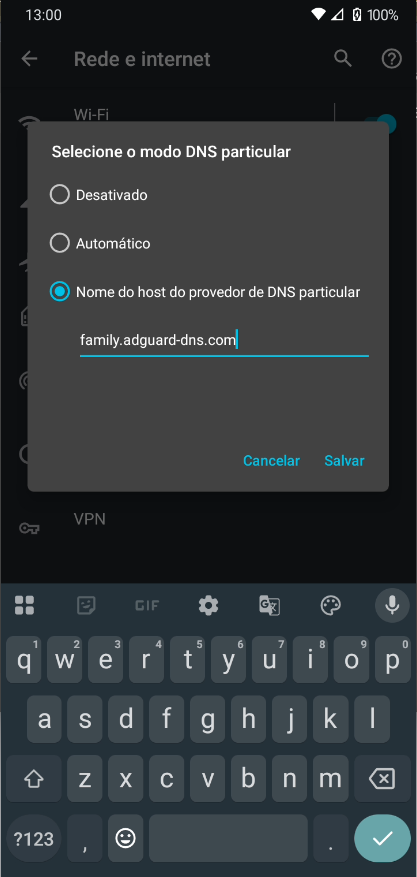
\includegraphics[width=0.8\textwidth]{../../assets/screenshots/print_dns.png}
    \textit{[Espaço reservado para o print do celular]}
\end{center}

\end{document}